\documentclass[tikz, border=3mm]{standalone}
\usepackage{tikz-3dplot} %pra plotar 3d
\usepackage{amsmath, amssymb}
\usetikzlibrary{calc,angles,quotes,arrows.meta, arrows, intersections} % Calc é necessário para parametrizar o arco
% Arrows.meta precisa pra mudar fazer alterações no tamanho da flecha/ponta do vetor
\usepackage{esint} % various fancy integral symbols
\usepackage{graphicx}
%%%%%%%Para fazer fluxograma%%%%%%%%%%5
\usetikzlibrary{shapes.geometric, arrows} 
\tikzstyle{startstop} = [rectangle, rounded corners, minimum width=3cm, minimum height=1cm,text centered, draw=black, fill=red!30]
\tikzstyle{io} = [trapezium, trapezium left angle=70, trapezium right angle=110, minimum width=3cm, minimum height=1cm, text centered, draw=black, fill=blue!30]
\tikzstyle{process} = [rectangle, minimum width=3cm, minimum height=1cm, text centered, draw=black, fill=orange!30]
\tikzstyle{decision} = [diamond, minimum width=3cm, minimum height=1cm, text centered, draw=black, fill=green!30]
\tikzstyle{arrow} = [thick,->,>=stealth]

%\lstset{style=mystyle}
%\author{Matheus Roos}
%\title{8 formas de escrever um programa em Fortran}
%\date{\today}

\begin{document}

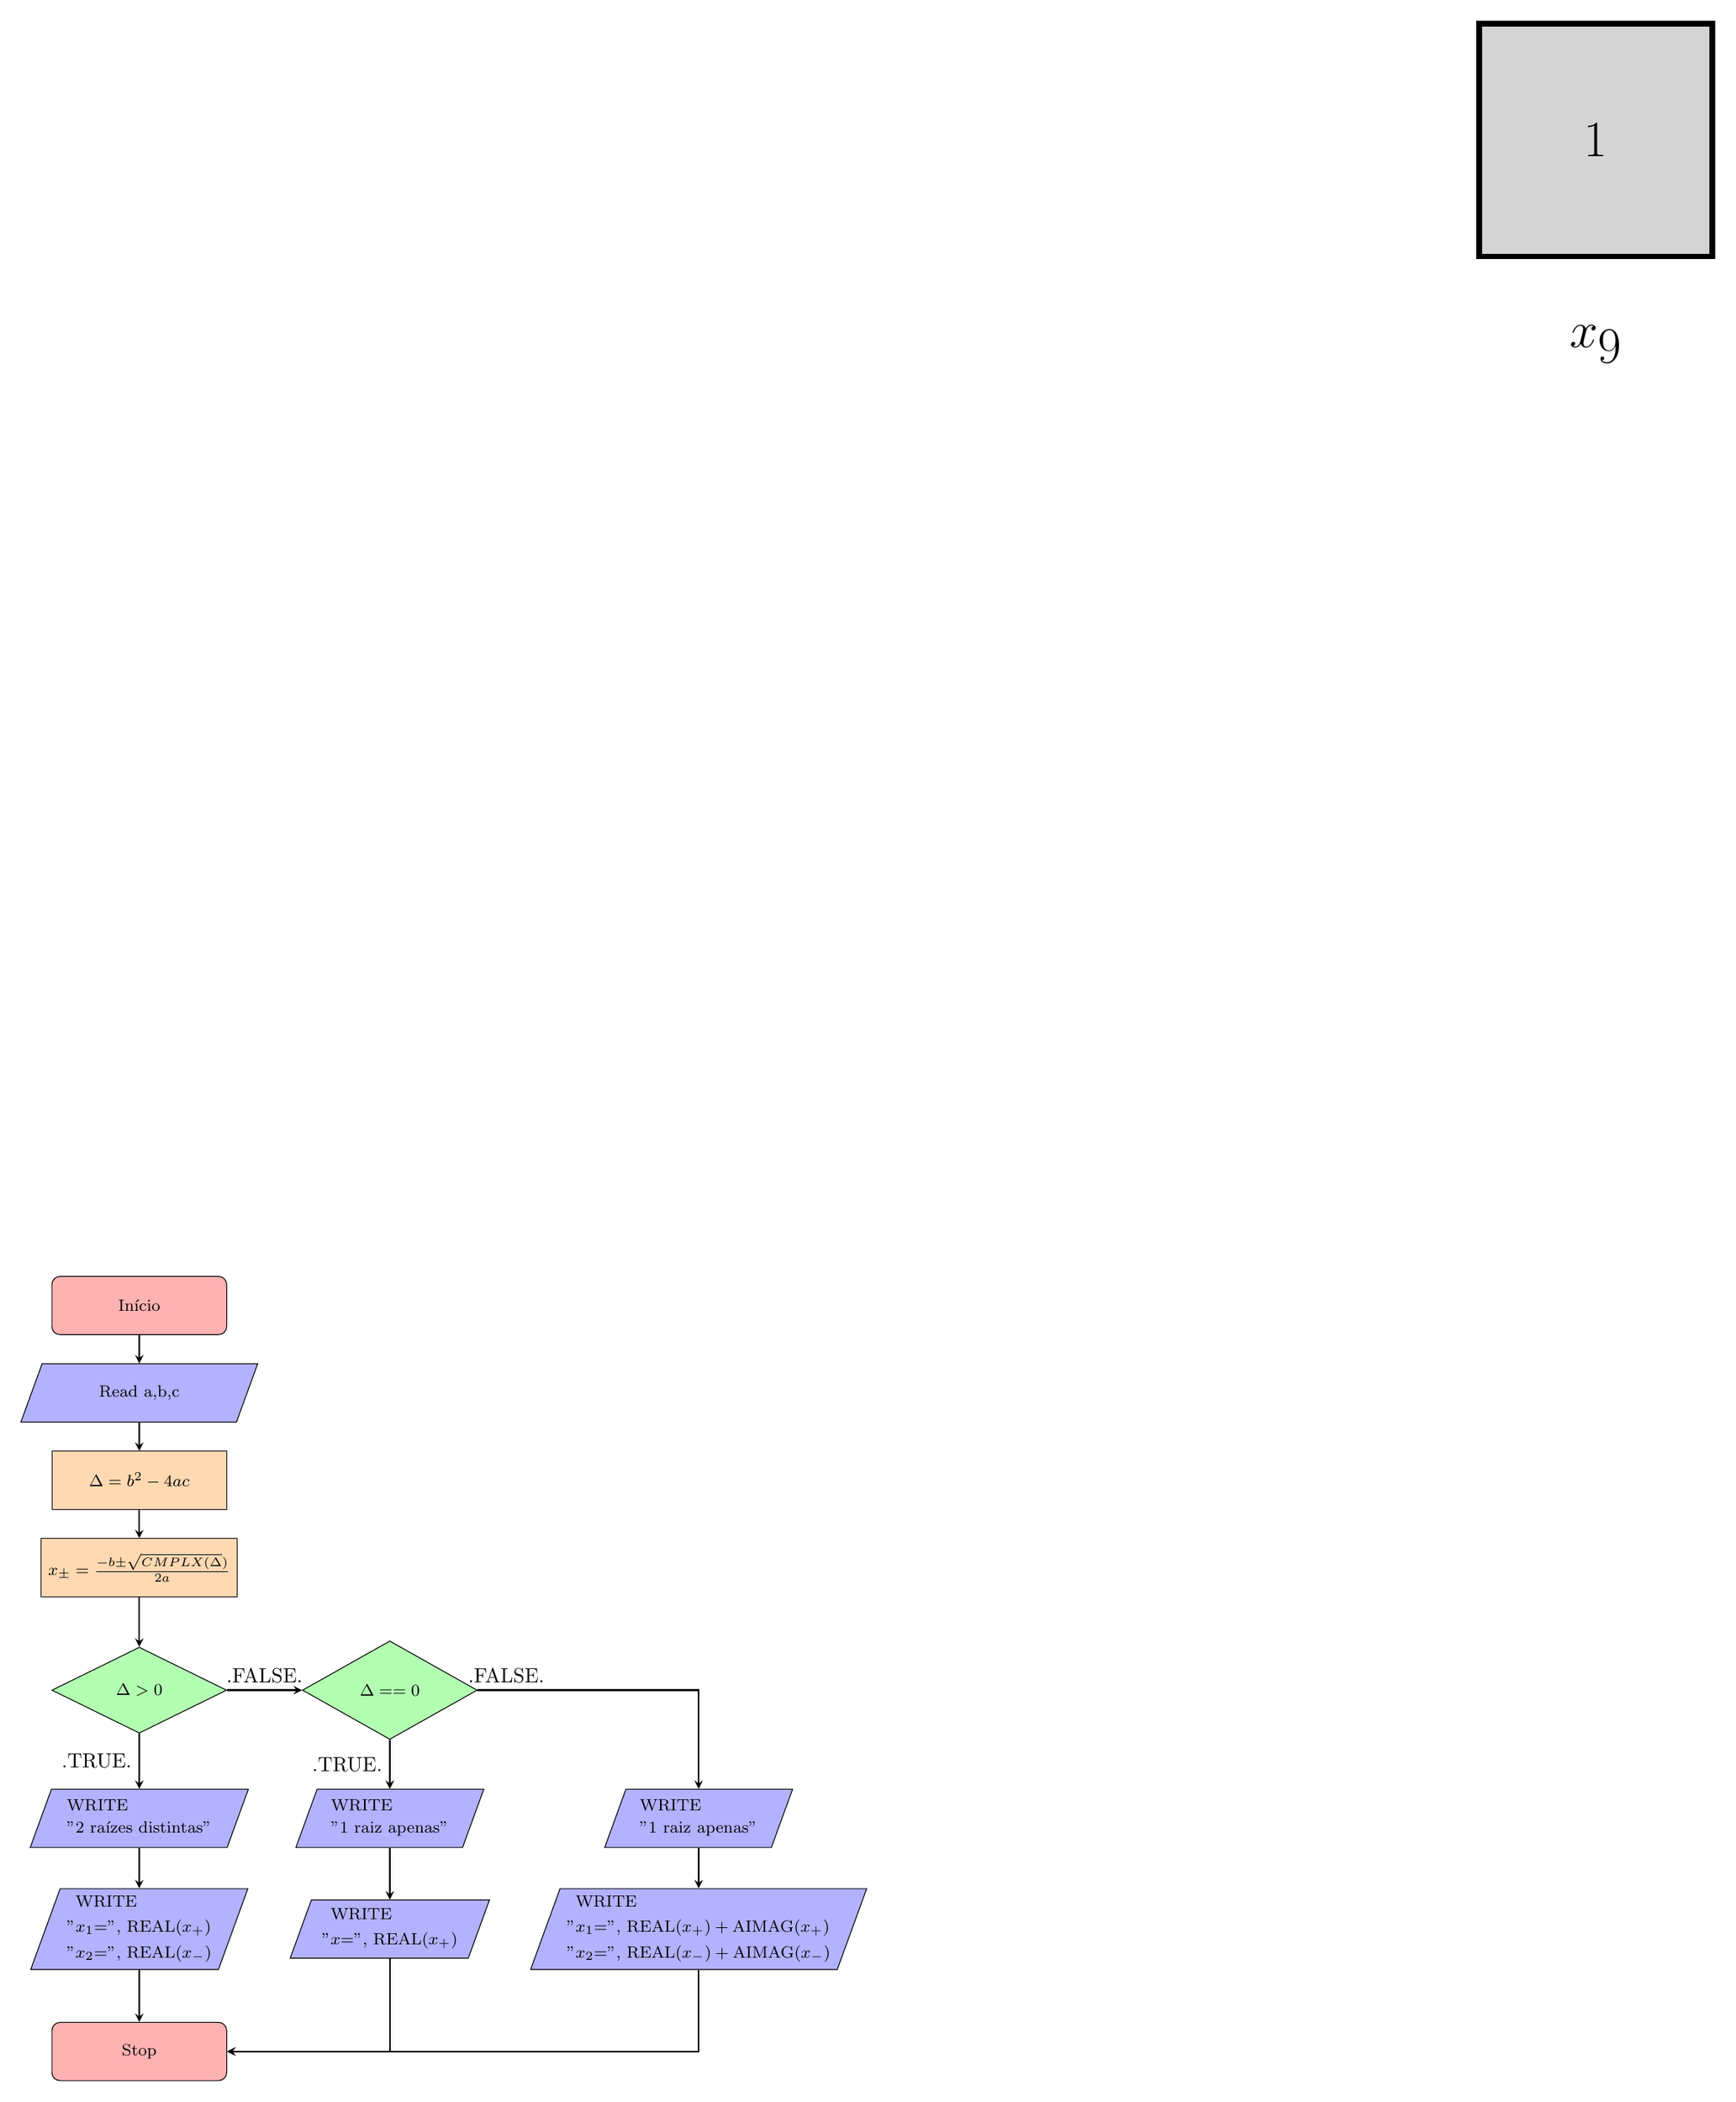
\begin{tikzpicture}[node distance=2.2cm]
%background
\draw node[draw, fill={{rgb:black,1;white,5}}, minimum size=4cm,line width=0.1cm,font=\fontsize{100}{100}\selectfont, label={[yshift=-6cm,style={font=\fontsize{100}{100} } ] {$x_9$} } ] at (25, 20) {1};
%nodes
%Início
\node[font=\fontsize{8pt}{8pt}\selectfont] (start) [startstop] {Início};
\node[font=\fontsize{8pt}{8pt}\selectfont] (in1) [io, below of=start, yshift=.7cm] {Read a,b,c};
\node[font=\fontsize{8pt}{8pt}\selectfont] (pro1) [process, below of=in1, yshift=.7cm] {$\Delta = b^{2} - 4ac$};
\node[font=\fontsize{8pt}{8pt}\selectfont] (pro1b) [process, below of=pro1, yshift=.7cm] {$x_{\pm} = \frac{-b \pm\sqrt{CMPLX(\Delta})}{2a}$};

%Duas raízes distintas
\node[font=\fontsize{8pt}{8pt}\selectfont] (dec1) [decision, below of=pro1b, yshift=.1cm] {$\Delta>0$};
\node[font=\fontsize{8pt}{8pt}\selectfont] (pro2a) [io, below of=dec1] {$\begin{aligned} & \text{WRITE} \\ & \text{"2 raízes distintas"}\end{aligned}$};
\node[font=\fontsize{8pt}{8pt}\selectfont] (pro2b) [io, below of=pro2a, yshift=.3cm] {$\begin{aligned} 
	& \text{WRITE} \\ \text{"} 
	& x_{1} \text{=", } \text{REAL(} x_{+} \text{)} \\ \text{"} 
	& x_{2} \text{=", } \text{REAL(} x_{-} \text{)}
\end{aligned}$};

%%%%%%%%%%%Apenas uma raiz
\node[font=\fontsize{8pt}{8pt}\selectfont] (dec2) [decision, right of=dec1, xshift=2.1cm] {$\Delta == 0$};
\node[font=\fontsize{8pt}{8pt}\selectfont] (in1sub) [io, below of=dec2] {$\begin{aligned} & \text{WRITE} \\ & \text{"1 raiz apenas"}\end{aligned}$};
\node[font=\fontsize{8pt}{8pt}\selectfont] (pro1sub) [io, below of=in1sub, yshift=.3cm] {$\begin{aligned} 
	& \text{WRITE} \\ \text{"} 
	& x \text{=", } \text{REAL(} x_{+} \text{)}
	\end{aligned}$};
%%%%%%%%%%%%%%%%%% Duas raízes complexas
\node[font=\fontsize{8pt}{8pt}\selectfont] (pro3) [io, right of=in1sub, xshift=3.1cm] {$\begin{aligned} & \text{WRITE} \\ & \text{"1 raiz apenas"}\end{aligned}$};

\node[font=\fontsize{8pt}{8pt}\selectfont] (pro3b) [io, below of=pro3, yshift=.3cm] {$\begin{aligned} 
	& \text{WRITE} \\ \text{"} 
	& x_{1} \text{=", } \text{REAL(} x_{+} \text{)} + \text{AIMAG(} x_{+} \text{)} \\ \text{"} 
	& x_{2} \text{=", } \text{REAL(} x_{-} \text{)}  + \text{AIMAG(} x_{-} \text{)}
	\end{aligned}$};
%Finalizando
\node[font=\fontsize{8pt}{8pt}\selectfont] (stop) [startstop, below of=pro2b, yshift=.1cm] {Stop};

%arrows
\draw [arrow] (start) -- (in1);
\draw [arrow] (in1) -- (pro1);
\draw [arrow] (pro1) -- (pro1b);
\draw [arrow] (pro1b) -- (dec1);
%Duas raízes reais distintas
\draw [arrow] (dec1) -- node[anchor=east] {.TRUE.} (pro2a);
\draw [arrow] (pro2a) -- (pro2b);
%Apenas uma raiz
\draw [arrow] (dec1) -- node[anchor=south] {.FALSE.} (dec2);
\draw [arrow] (dec2) -- node[anchor=east] {.TRUE.} (in1sub);
\draw [arrow] (in1sub) -- (pro1sub);
%Duas raízes complexas
\draw [arrow] (dec2) node[anchor=south, xshift=2.cm] {.FALSE.} -|  (pro3);
\draw [arrow] (pro3) -- (pro3b);
%Finalizando
\draw [arrow] (pro2b) -- (stop);
\draw [arrow] (pro3b) |- (stop);
\draw [arrow] (pro1sub) |- (stop);
\end{tikzpicture}

 
\end{document}
